%% uctest.tex 11/3/94
%% Copyright (C) 1988-2004 Daniel Gildea, BBF, Ethan Munson.
%
% This work may be distributed and/or modified under the
% conditions of the LaTeX Project Public License, either version 1.3
% of this license or (at your option) any later version.
% The latest version of this license is in
%   http://www.latex-project.org/lppl.txt
% and version 1.3 or later is part of all distributions of LaTeX
% version 2003/12/01 or later.
%
% This work has the LPPL maintenance status "maintained".
% 
% The Current Maintainer of this work is Daniel Gildea.
%
% 2007/08/01
% LaTeX Package "ucr" is modified from LaTeX package "ucthesis."
% This modification is therefore under to the conditions of 
% the LaTeX Project Public License.
% Its formality is suitable for the dissertation of Universty of
% California, Riverside.
% This test document is for the convenience of all students of
% Universty of California, Riverside.
% Contact Charles Yang at chcyang@yahoo.com if you like.
% Charles Yang has nothing to do with the original author's sarcasm.
%
% \documentclass[11pt]{ucthesis}
% \documentclass[11pt]{ucr}
\documentclass[oneside,final, letterpaper]{ucr}
\usepackage[backend=biber,sortcites=true]{biblatex}
\addbibresource{bibfile.bib}
\usepackage{tikz}
\usetikzlibrary{math}
\usetikzlibrary{arrows.meta}
\usetikzlibrary{positioning}
\usepackage{ifthen}
\tikzset{>={Stealth[length=1.25mm]}}
\newcommand{\todocite}{{\color{red}CITE}}
\newcommand{\todo}[1]{{\color{red}TODO: #1}}
\usepackage{siunitx}
\begin{document}

% Declarations for Front Matter

\title{The Title of Your Thesis Goes Here}
\author{Clarity Laska Shimoniak}
\degreemonth{March}
\degreeyear{2024}
\degree{Master of Science}
\chair{Dr. Philip Brisk}
\othermembers{Dr. Daniel Wong\\
Dr. Ahmed Eldawy}
\numberofmembers{3}
\field{Computer Engineering}
\campus{Riverside}

\maketitle
\copyrightpage{}
\approvalpage{}

\degreesemester{Fall}

\begin{frontmatter}

\begin{acknowledgements}
I am grateful to my advisor Philip Brisk, without whose guidance, feedback,
support, and advocacy I would not have be here.

I am grateful to Prithviraj Yuvaraj, whose support on the navigating Vitis HLS
and the OCT testbed have been invaluable to my engineering efforts.

I am grateful to my friends in Kansas for telling me about Zotero to keep track
of all my references..
\end{acknowledgements}

\begin{dedication}
\null\vfil
{\large
\begin{center}
To my friends for keeping me sane, and to their cats for helping me smile.
\end{center}}
\vfil\null
\end{dedication}

\begin{abstract}
% Abstract should be double-spaced and limited to 350 words or 2,450 characters.
Both FPGAs and RDMA have seen increasing adoption in datacenters as a means of achieving the parallelism and responsiveness needed in modern applications. We propose a novel database architecture built around a distributed FPGA cluster with RDMA as its interconnect in order to implement high-performance, in-memory key-value store based on the B-Link tree.
\end{abstract}


\tableofcontents
\listoffigures
\listoftables
\end{frontmatter}

% \part{First Part}


\chapter{Introduction}

Introduction goes here
 %usually intro
\sect{Overview}

\subsect{Database Indexing}
\label{sec:indexing}

It is common for modern databases to use a variant of the B-Tree for indexing
\autocite{ma-tpds-2022}. Shorter trees yield faster lookups, as lookup time is
proportional to the length of the path from the root node where the search
begins to the node holding the desired data. The self-balancing nature of
B-Trees helps to control the height of the tree and thus lookup times. B+ trees
are a variant of B trees the keep all data values at the leaves rather than
storing them alongside internal nodes, which improves the average case time of
tree traversal in terms of number of I/O operations.

B-Link trees are an extension to B+ trees proposed by \citeauthor{b-link} in
\citeyear{b-link} which add fields to provide for thread-safe access. Like B+
trees, they are self-balancing, have an adjustable fan-out factor, and store all
data at leaf nodes. B-Link trees introduce linkages between sibling nodes at all
levels of the tree. Principally, this is to ensure that newly created sibling
nodes are still accessible during split operations, even if they have not yet
been assigned to a parent node. This structure ensures that no more than three
nodes are locked at a time for each modification operation. However, this also
brings the benefit that range-based queries can be executed very easily, as
subsequent leaf nodes form a linked list \autocite{b-link}.


\subsect{FPGAs}
\label{sec:fpga}

Field-Programmable Gate Arrays (FPGAs) are an alternative processing element to
CPUs. Structurally, FPGAs are large arrays of reconfigurable logic gates that
can be used to implement complex digital circuits. This lower-level approach
allows for designs to exploit more parallelism than CPUs. FPGAs will not perform
as well as application-specific integrated circuits (ASICs) for an identical
design, but on-demand reconfigurability, shorter lead times, and lower cost (for
all but the largest order sizes) offsets these downsides in many applications.

A key difference of FPGAs from CPUs is how computational resources are
multiplexed. On CPU-based systems, computational resources are multiplexed
temporally; there are a limited number of instructions that can be executed each
second. FPGAs are multiplexed spatially; all processes can run simultaneously so
long as there are sufficient gates available to implement them.

Traditionally, FPGA designs are written in hardware description languages
(HDLs), with the two most prominent being Verilog and VHDL. However, in recent
years attempts have been made to change this. High-Level Synthesis (HLS)
frameworks convert programs written in traditional programming languages like C
\& C++ into HDL. This allows for easier conversion of existing algorithms and
codebases as well as increasing the pool of potential developers
\autocite{martin-destest-2009}. More recently, projects like Chisel seek to blur
the line by modifying an existing programming language, Scala, to support HDL
semantics \autocite{chisel}.

Originally, FPGAs were intended for prototyping ASICs, but later found wide
usage in the telecom industry \autocite{bobda-trets-2022,mencer-queue-2020} and
more recently in datacenters \autocite{mencer-queue-2020,hoozemans-cas-2021}.
FPGAs are uniquely suited to networking applications because the dataflow
programming model \autocite{hoozemans-cas-2021} inherent to their architecture
aligns naturally with the flow of packets in high-throughput networking
environments \autocite{mueller-sigmod-2009}.


\subsect{FPGAs in the Datacenter}
\label{sec:datacenter-fpga}

FPGA implementations of many core database operations have been developed.
Converting algorithms from CPU to FPGA is fairly straightforward
\autocite{fang-vldb-2020}, especially with the help of HLS, but optimizing them
is a focus of ongoing research \autocite{fang-vldb-2020}. Converting simple
operations like filter and projection (removing some columns from a table before
returning it) are largely a solved problem \autocite{fang-vldb-2020}, but more
complicated operations like merge and sort have been implemented in many ways,
with some showing significant performance improvements over CPU versions
\autocite{leggett-trets-2025,moghaddamfar-damon-2021}.

Much of the recent research into using FPGAs for database acceleration focuses
on specialized Network Interface Cards (NICs) called SmartNICs. These contain a
small FPGA, which allows for some processing to be offloaded from the CPU at the
point of access to the network. However, the smaller program space and reduced
performance of these FPGAs limit how much work can be moved onto them from other
parts of the system. For instance, \citetitle{honeycomb} chooses to only
accelerate read operations, assuming a read-heavy workload \autocite{honeycomb}.
The structure of FPGAs incentivizes prioritizing common, simple operations
because of the resource multiplexing issues mentioned above
\autocite{honeycomb,moghaddamfar-damon-2021}.

\sect{System Architecture}

\subsect{Comparison with \citeauthor{base}}

Our design is based on that of \citeauthor{base} in \citetitle{base}. Their
design uses a CPU cluster with an RDMA interconnect. The design follows the
Network-Attached-Memory (NAM) architecture, where some nodes are dedicated to
computation while others are dedicated to storage
\autocite{base,binnig-vldb-2016}.

For indexing, they use an adaptation of the B-link tree with a sliding scale of
distribution schemes. At one end is the coarse-grained scheme, where entries are
assigned to nodes based on ranges or hashes of their keys. This allows for fast
traversal at the cost of poor bandwidth utilization, as bulk accesses to ranges
of data must all be served from one node. At the other end is the fine-grained
scheme, where new values are written to nodes in around-robin manner. This
improves bandwidth utilization by allowing all nodes to access memory
simultaneously, but slows down the initial lookup process. Finally, they propose
a hybrid scheme which uses coarse-grained for the top of the tree and
fine-grained for the leaves, attempting to maximize the benefit of each strategy
\autocite{base}.

To support concurrent access, their design uses optimistic lock coupling rather
than traditional lock coupling. This strategy does not protect areas from
concurrent access, but simply identifies when data has been changed. If two
writers begin modifying the same data, the one who writes back to main memory
second will see that its version is not what was expected, and attempt to
restart its operation using this new data. A key advantage of this strategy is
reducing cache misses due to cache invalidations that result when frequently
writing to lock bits in main memory on multi-core CPUs
\autocite{leis-damon-2016}. On an FPGA, we have the freedom to design our own
caching protocol rather than mimic the general purpose caching protocols that
are fixed in the silicon of CPUs. Thus, this problem could be negated by
managing lock bits differently from other memory to reduce caching overhead
rather than avoiding writes altogether. As noted by
\citeauthor{binnig-vldb-2016}, DBMSs function best with full control over memory
management \autocite{binnig-vldb-2016}.


\subsect{Memory Layout}

A key challenge of converting the design proposed by \citeauthor{base} from CPU
to FPGA is that all memory must be managed manually; there is no operating
system or standard library to dynamically allocate memory or handle virtual
addressing. This makes it desirable for addresses of nodes within a tree to
change as little as possible, as without an internal address translation layer,
any movement of a node within a cluster would require that address change to be
broadcast to all other nodes in the cluster with links to it.

\newcommand{\clusternode}[1]{
	% Cluster Boundary
	\draw ({(#1)*6}, 0) ++(-2.75, 0.5) rectangle ++(5.5, -3);
	% Tree Nodes
	\node[tree] at ({(#1)*6}, 0) (n#1 00) {};
	% Rows
	\foreach \r [
		evaluate = \r as \w using int(3^\r),
		evaluate = \r as \wl using int(3^\r-1)
	] in {1,...,2} {
		% Columns
		\foreach \c [
			evaluate = \c as \i using int((\w-1)/2 + \c-1),
			evaluate = \c as \pr using int(\r-1),
			evaluate = \c as \pc using int(\c/3),
			evaluate = \c as \cl using int(\c-1)
		] in {0,...,\wl} {
			\node[tree] (n#1 \r\c)
				at ({(#1)*6 + (\c-int(\w/2)) / (\w/5)}, -\r) {};
			\draw[->] (n#1 \pr\pc) -- (n#1 \r\c);
			\ifthenelse{\c=0}{}{
				\draw[->] (n#1 \r\cl) -- (n#1 \r\c);
			}
		}
	}
}

\begin{figure}
	\centering
	\begin{tikzpicture}[
		scale=0.7,
		tree/.style={draw,circle,inner sep=0.5mm}
	]
		\clusternode{0}
		\clusternode{1}
		\draw[->] (n0 00) -- (n1 00);
		\draw[->] (n0 12) -- (n1 10);
		\draw[->] (n0 28) -- (n1 20);
	\end{tikzpicture}
	\caption{Linkages Between Sub-Trees in the Cluster}
\label{coarse-link}
\end{figure}

The most straightforward memory layout is the one shown in figure
\ref{coarse-link}, analogous to \citeauthor{base}'s coarse grained distribution.
A sub-tree corresponding to a range of entries is allocated to each node in the
cluster. This allows each tree to operate independently from others in most
cases \autocite{ma-tpds-2022}, allowing greater flexibility to manage its own
memory. This also imposes a worst-case number of links between nodes as the
height of each sub-tree.

\sect{Experiment}

\begin{figure}
	\centering
	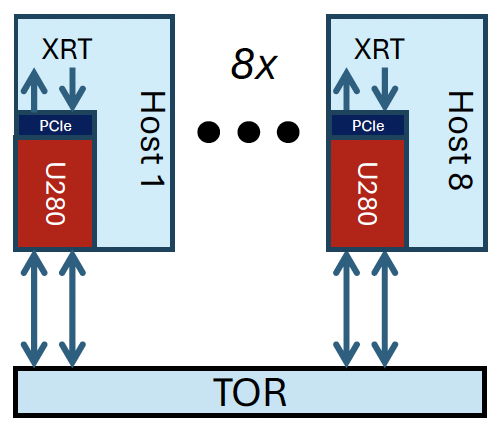
\includegraphics[width=2in]{oct-arch.jpg}
	\caption{Cluster Architecture}
	\label{oct-arch}
\end{figure}

The database was implemented on a cluster of 8 nodes that share a single network switch as shown in figure \ref{oct-arch}. Each node has a Xilinx Alveo U280 PCIe card, containing a XCU280 FPGA and $\SI{8}{\giga\byte}$ of high-bandwidth memory (HBM). Each node is connected to the switch with a $\SI{100}{\giga\bit}$ NIC.

\sect{Related Works}

\subsect{In Software}

\citeauthor{dlsm} propose using Log-Structured Merge Trees as a
higher-performance alternative to B-trees. However, their system architecture
assumes a heterogeneous cluster with some nodes dedicated to memory and other
dedicated to processing \autocite{dlsm}.


\subsect{Hardware Acceleration}

\citeauthor{star} have shown the viability of FPGAs as network accelerators, but
use them to implement custom a NIC protocol rather than as part of an
application \autocite{star}.

Utilizing more of the U280's memory hierarchy that could be leveraged for some
of these caching effects. In addition to the $\SI{8}{\giga\byte}$ of HBM used in
this experiment, it has $\SI{32}{\giga\byte}$ of slower, off-chip DDR and
$\SI{41}{\kilo\byte}$ of faster, on-chip block RAM (BRAM) and UltraRAM (URAM).

\citetitle{honeycomb} uses a hybrid approach, with CPU handling modification
operations and an FPGA-based smart NIC handling lookup operations. The main
reason that \citeauthor{honeycomb} give for this approach is that the cost of
accelerating modification operations was too high due to their complexity to be
beneficial in read-dominated workloads \autocite{honeycomb}. The U280 that we
are using is more capable than Honeycomb's embedded FPGA, so ``program space''
is not as much of a concern. Using Vitis HLS allows for these more complex
procedures to be described in a traditional software context, lowering the
amount of effort required to implement them effectively.

\section{Conclusions}

Conclusions go here




\nocite{*}
% \singlespacing
% \bibliographystyle{alpha}
\printbibliography

../common/appendix.tex


\end{document}
